\documentclass[12pt,a4paper]{article}
\usepackage[utf8]{inputenc}
\usepackage{amsmath}
\usepackage{amsfonts}
\usepackage{amssymb}
\usepackage{graphicx}
\usepackage{hyperref}
\usepackage{booktabs}
\usepackage{listings}
\usepackage{xcolor}
\usepackage{tikz}
\usetikzlibrary{shapes.geometric, arrows.meta, positioning, shadows}

\definecolor{codegreen}{rgb}{0,0.6,0}
\definecolor{codegray}{rgb}{0.5,0.5,0.5}
\definecolor{codepurple}{rgb}{0.58,0,0.82}
\definecolor{backcolour}{rgb}{0.95,0.95,0.92}
\definecolor{navyblue}{rgb}{0.0, 0.0, 0.5}

\hypersetup{
    colorlinks=true,
    linkcolor=navyblue,
    filecolor=magenta,      
    urlcolor=cyan,
    pdftitle={Flyhigh Technical Report},
    pdfpagemode=FullScreen,
}

\lstdefinestyle{mystyle}{
    backgroundcolor=\color{backcolour},   
    commentstyle=\color{codegreen},
    keywordstyle=\color{magenta},
    numberstyle=\tiny\color{codegray},
    stringstyle=\color{codepurple},
    basicstyle=\ttfamily\footnotesize,
    breakatwhitespace=false,         
    breaklines=true,                 
    captionpos=b,                    
    keepspaces=true,                 
    numbers=left,                    
    numbersep=5pt,                  
    showspaces=false,                
    showstringspaces=false,
    showtabs=false,                  
    tabsize=2
}
\lstset{style=mystyle}

\tikzset{
    startstop/.style={rectangle, rounded corners, minimum width=3.5cm, minimum height=1cm, text centered, draw=blue!50!black, fill=blue!10, very thick, drop shadow},
    process/.style={rectangle, minimum width=3.5cm, minimum height=1cm, text centered, draw=orange!50!black, fill=orange!10, very thick, drop shadow},
    decision/.style={diamond, aspect=1.5, minimum width=3cm, minimum height=1.5cm, text centered, draw=green!50!black, fill=green!10, very thick, drop shadow},
    io/.style={trapezium, trapezium left angle=70, trapezium right angle=110, minimum width=3.5cm, minimum height=1cm, text centered, draw=purple!50!black, fill=purple!10, very thick, drop shadow},
    arrow/.style={thick, -{Stealth[scale=1.2]}, draw=gray!60!black}
}

\title{\textbf{Flyhigh: Premium Airline Booking \& Operations System} \\ \large Complete End-to-End Technical Documentation \& Systems Architecture}
\author{\textbf{Software Engineering Division} \\ System Architecture \& Core Development Documentation}
\date{\today}

\begin{document}

\maketitle

\begin{abstract}
This comprehensive technical report details the design, engineering, database architecture, and implementation of \textbf{Flyhigh}, a premium full-stack web application tailored for modern flight bookings and operational fleet management. The solution employs a responsive client frontend engineered with React (Vite) and Tailwind CSS, an API service layer powered by Node.js and Express, and a robust persistence tier supported by MongoDB. The report outlines key architectural components, including a combinatorial flight schedule generator, secure Stripe checkout sessions with crash-resilient fallback pipelines, dynamic passenger manifesting, and a state-of-the-art admin control panel for supervising schedules, passenger listings, bookings, feedback telemetry, and fleet profiles.
\end{abstract}

\newpage
\tableofcontents
\newpage

\section{Introduction}
Modern civil aviation systems demand web architectures that balance rich client interactions with transactional data integrity. The \textbf{Flyhigh} platform addresses these operational necessities by establishing a seamless integration between passenger-facing booking screens and administrative oversight components. 

The primary capabilities and implementation objectives accomplished in this project include:
\begin{itemize}
    \item \textbf{Immersive Glassmorphic UI}: Constructing a premium client interface using React and Tailwind CSS that utilizes custom backdrops, shadows, and clean typography.
    \item \textbf{Stripe Payment Infrastructure}: Configuring checkout redirections via Stripe checkout APIs, supplemented with dry-run/sandbox fallback mechanics to prevent crashes when API keys are absent or invalid.
    \item \textbf{Dynamic Multi-Passenger Processing}: Collecting passenger details concurrently, computing comprehensive price breakdowns (including seat premium tiers, processing fees, and taxes), and printing structured e-tickets with mock barcode graphic layouts.
    \item \textbf{Administrative Oversight (SSO Portal)}: Delivering a comprehensive administrative dashboard for managing airlines, defining flight route catalogs, updating real-time flight schedules/capacities, auditing passenger manifests, monitoring user profiles, and analyzing feedback reviews.
    \item \textbf{Database Persistence \& Scheduling Seeding}: Utilizing MongoDB to establish collections and running combinatorial algorithms to generate realistic flight networks and timetables across key airport hubs.
\end{itemize}

\section{System Architecture}
The application follows a modular three-tier architecture (Client, Application, and Database), structured to run locally on dedicated communication ports.

\begin{figure}[htbp]
\centering
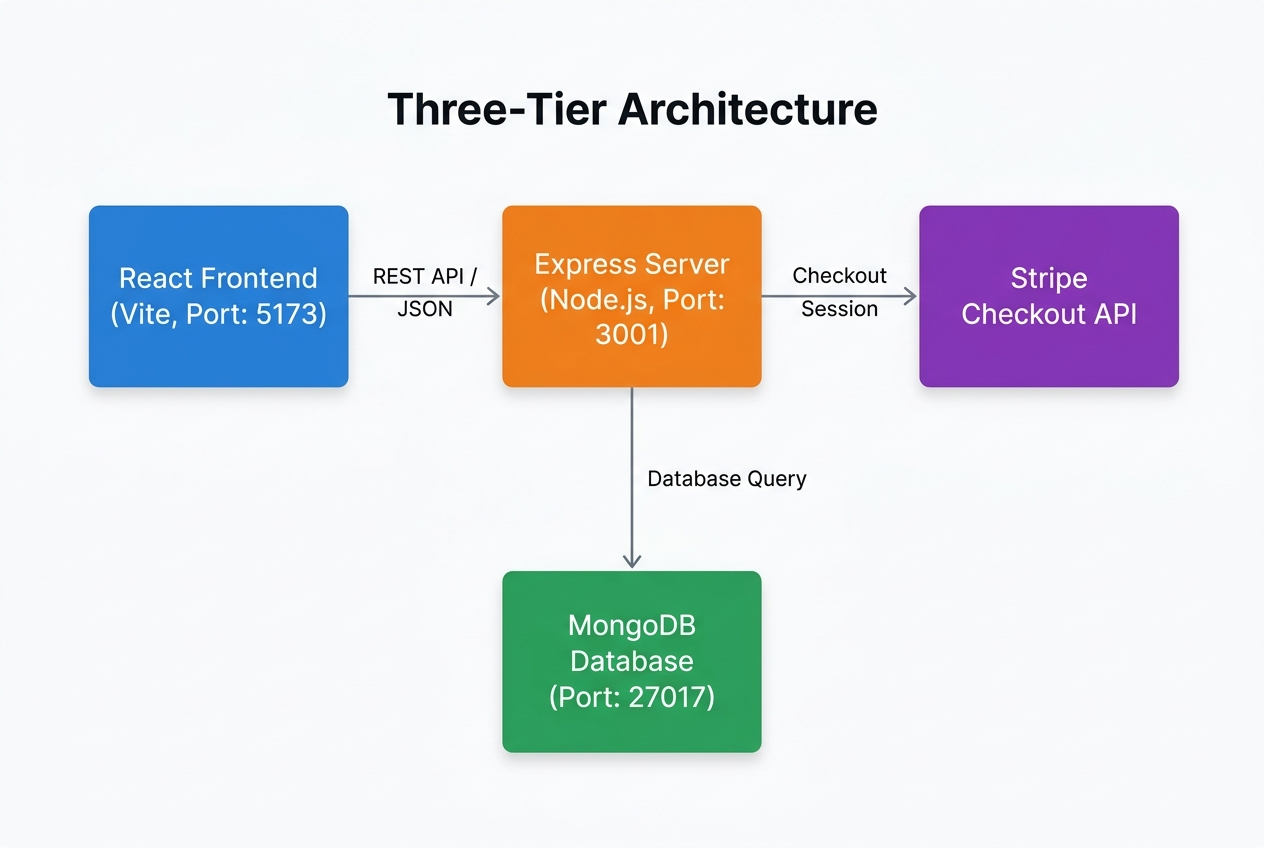
\includegraphics[width=0.9\textwidth]{images/architecture_diagram.jpg}
\caption{Three-Tier Architecture Diagram with Communication Channels}
\label{fig:architecture}
\end{figure}

\subsection{Frontend Tier (Client Engine)}
The user interface is a Single Page Application (SPA) built with React.js. It features:
\begin{itemize}
    \item \textbf{Vite Build Tool}: Powering extremely rapid hot-module replacement and clean asset bundling.
    \item \textbf{React Router DOM}: Implementing client-side routing across a wide list of endpoints for both the main client app and the admin portal.
    \item \textbf{React-to-Print Hooks}: Allowing high-fidelity boarding pass structures to print cleanly to physical sheets or PDFs.
\end{itemize}

\subsection{Backend Tier (Application Logic)}
The backend services run on Node.js utilizing Express.js. Key design principles include:
\begin{itemize}
    \item \textbf{CORS Enablement}: Configuring custom origins to enable cross-domain requests between client and server ports.
    \item \textbf{Configured Security Listeners}: Establishing process handlers to capture unexpected errors and reject issues gracefully before they terminate the Node process.
    \item \textbf{Environment Isolation}: Utilizing an isolated config file (\texttt{backend/env.txt}) to manage MongoDB URIs and Stripe secret keys.
\end{itemize}

\subsection{Database Tier (Persistence Engine)}
The database uses MongoDB. A native client driver handles queries, updates, and inserts inside standard API controllers. Connections are handled through standard connection pools.

\newpage
\section{Database Schema \& Data Architecture}
The system establishes a dedicated MongoDB database named \texttt{Airline}. The configuration is saved inside \texttt{backend/env.txt}. The schema consists of six core collections:

\subsection{Airlines Collection}
Tracks airline fleet codes, carrier designations, and array of flight numbers:
\begin{itemize}
    \item \texttt{\_id}: MongoDB ObjectId.
    \item \texttt{airlineName}: String (e.g., "Air India").
    \item \texttt{flightCode}: String (e.g., "AI").
    \item \texttt{flights}: Array of Strings containing assigned flight numbers.
\end{itemize}

\subsection{Airports Collection}
Stores lists of serving domestic flight hubs:
\begin{itemize}
    \item \texttt{code}: String (e.g., "DEL").
    \item \texttt{name}: String (e.g., "Delhi").
    \item \texttt{city}: String (e.g., "New Delhi").
    \item \texttt{country}: String (e.g., "India").
\end{itemize}

\subsection{Flights Collection}
Serves as the global flight catalog of active flight routes:
\begin{itemize}
    \item \texttt{flightName}: String (e.g., "SpiceJet").
    \item \texttt{flightNumber}: String (e.g., "SG103").
    \item \texttt{originAirport}: String (e.g., "BOM").
    \item \texttt{destinationAirport}: String (e.g., "MAA").
\end{itemize}

\subsection{Flight Info Collection}
Manages date-specific departure slots, ticket pricing grids, and active seating numbers:
\begin{itemize}
    \item \texttt{flightNumber}: String (e.g., "AI101").
    \item \texttt{departureDate}: String (e.g., "2026-08-08").
    \item \texttt{departureTime}: ISO Timestamp String (e.g., "2026-08-08T06:00").
    \item \texttt{arrivalTime}: ISO Timestamp String (e.g., "2026-08-08T08:15").
    \item \texttt{prices}: Nested Object holding pricing tiers:
    \begin{itemize}
        \item \texttt{economy}: Number (INR).
        \item \texttt{business}: Number (INR).
        \item \texttt{first}: Number (INR).
    \end{itemize}
    \item \texttt{seatsAvailable}: Nested Object holding cabin capacities:
    \begin{itemize}
        \item \texttt{economy}: Number (Default: 60).
        \item \texttt{business}: Number (Default: 12).
        \item \texttt{first}: Number (Default: 4).
    \end{itemize}
\end{itemize}

\subsection{Bookings Collection}
Compiles successfully processed travel itineraries and passenger manifests:
\begin{itemize}
    \item \texttt{email}: String (Customer login email).
    \item \texttt{time}: ISO Timestamp (Booking timestamp).
    \item \texttt{data}: Flight details (flight number, date, cabin seat class, price).
    \item \texttt{formData}: Array of Passenger Objects (Title, First Name, Last Name, Mobile, Seat).
\end{itemize}

\subsection{Users Collection}
Contains registered profiles and status flags:
\begin{itemize}
    \item \texttt{title}: String (e.g., "Mr.").
    \item \texttt{firstName}: String (First name).
    \item \texttt{lastName}: String (Last name).
    \item \texttt{email}: String (Unique identifier).
    \item \texttt{password}: String (Credentials).
    \item \texttt{mobileNumber}: String (Contact info).
    \item \texttt{status}: String (Active or Inactive status managed by Admin).
\end{itemize}

\subsection{Feedback Collection}
Tracks customer reviews:
\begin{itemize}
    \item \texttt{email}: String.
    \item \texttt{rating}: Number (1 to 5).
    \item \texttt{firstImpression}: String.
    \item \texttt{hearAbout}: String.
    \item \texttt{missingAnything}: String.
\end{itemize}

\newpage
\section{Backend REST API Reference}
The table below logs the fully implemented endpoints inside \texttt{backend/server.js}:

\begin{table}[h!]
\centering
\small
\begin{tabular}{lllp{6cm}}
\toprule
\textbf{HTTP Method} & \textbf{Endpoint} & \textbf{Payload Scope} & \textbf{Description} \\
\midrule
\texttt{GET} & \texttt{/api/airlines} & None & Fetch list of all registered airlines. \\
\texttt{POST} & \texttt{/api/airlines} & Airline data & Add new airline fleet parameters. \\
\texttt{POST} & \texttt{/api/airlines-addflt} & Flight code, number & Append flight numbers to carrier list. \\
\texttt{GET} & \texttt{/api/airports} & None & Retrieve domestic airports database. \\
\texttt{GET} & \texttt{/bookings} & None & Fetch list of all customer bookings. \\
\texttt{POST} & \texttt{/bookings} & Booking info & Insert new booking transaction record. \\
\texttt{POST} & \texttt{/api/login} & Email, Password & Verify customer credentials for login. \\
\texttt{POST} & \texttt{/api/users} & User profile & Register a new customer profile. \\
\texttt{POST} & \texttt{/api/update-profile} & Updated info & Update customer user registration. \\
\texttt{POST} & \texttt{/api/update-profile-on} & Email, Status & Change user account status flag. \\
\texttt{GET} & \texttt{/api/flights} & None & Fetch all active flight route catalog. \\
\texttt{POST} & \texttt{/api/flights} & Flight catalog item & Insert new flight route code. \\
\texttt{GET} & \texttt{/api/flights/count} & None & Aggregate flight count grouped by carrier. \\
\texttt{GET} & \texttt{/api/feedback} & None & Retrieve all feedback entries. \\
\texttt{POST} & \texttt{/api/feedback} & Review details & Insert new user experience rating. \\
\texttt{GET} & \texttt{/api/flightinfo} & None & Retrieve scheduled flights listings. \\
\texttt{POST} & \texttt{/api/flightinfo} & Flight code, Date & Fetch schedule for a flight on a date. \\
\texttt{POST} & \texttt{/api/flight} & Decr. passenger count & Decrement seat counts on booking completion. \\
\texttt{POST} & \texttt{/api/payments} & Purchase particulars & Create Stripe Checkout redirection session. \\
\bottomrule
\end{tabular}
\caption{API Services Directory and Endpoints Schema}
\label{tab:apis}
\end{table}

\newpage
\section{Customer Booking Flow \& Implementation}
The client site structures the booking process in a sequential, state-preserving pipeline:

\begin{figure}[htbp]
\centering
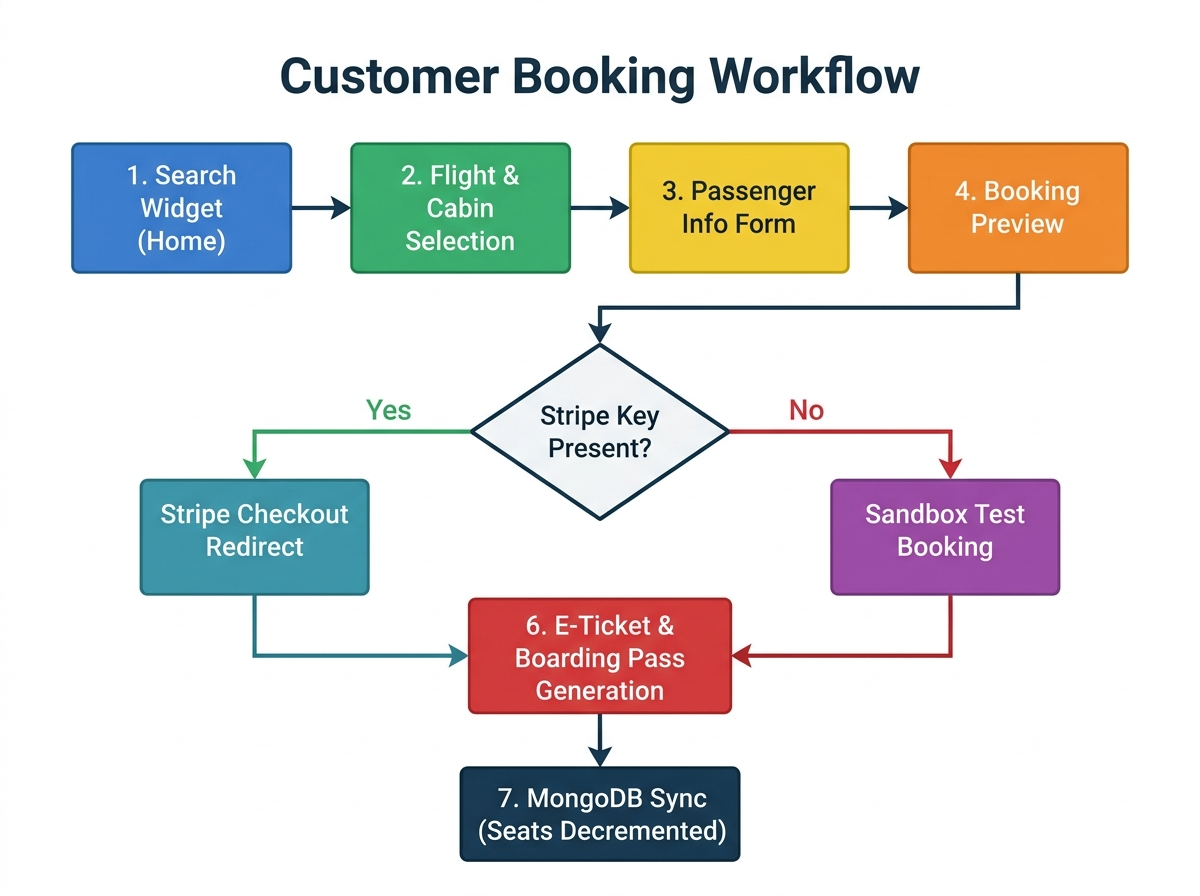
\includegraphics[width=0.9\textwidth]{images/booking_flow_chart.jpg}
\caption{Comprehensive Passenger Booking Process Workflow}
\label{fig:booking_flow}
\end{figure}

\subsection{Combinatorial Flight Network Seeding}
To establish realistic scheduling patterns, \texttt{seedFlights.js} runs a combinatorial algorithm across the four primary domestic hub nodes: Delhi (\texttt{DEL}), Mumbai (\texttt{BOM}), Chennai (\texttt{MAA}), and Kolkata (\texttt{CCU}). Using a 2-permutation formula:
\begin{equation}
P(n, r) = \frac{n!}{(n-r)!} = \frac{4!}{(4-2)!} = 12 \text{ distinct routes}
\end{equation}
With 3 operating carriers (Air India, IndiGo, and SpiceJet), this expands to $12 \times 3 = 36$ distinct route vectors. Seeding these routes over a rolling 3-day calendar window (Today, Tomorrow, and Day After) creates exactly 108 flight schedules, each pre-configured with distinct cabin class capacities (Economy: 60, Business: 12, First Class: 4).

\subsection{Dynamic Billing Calculations}
Before initiating payment redirection, \texttt{Preview.jsx} computes costs based on seat count and class selection:
\begin{equation}
\text{Base Cost} = \text{Passengers} \times \text{Class Fare}
\end{equation}
\begin{equation}
\text{Total Billing} = \text{Base Cost} + \text{Convenience Fee (350 INR)} + \text{GST (18\% of Base Cost)}
\end{equation}

\subsection{Seat Increment & Decrement Locking}
When a user completes payment and accesses their ticket pass, the frontend dispatches a decrement operation:
\begin{lstlisting}[language=javascript]
app.post("/api/flight", async (req, res) => {
  const { flightNumber, departureTime, seat, passengers } = req.body;
  const result = await collection.updateOne(
    { flightNumber, departureTime },
    { $inc: { [`seatsAvailable.${seat}`]: -passengers } }
  );
  res.send(result);
});
\end{lstlisting}
This prevents overbooking on subsequent seat queries.

\subsection{High-Fidelity E-Tickets & Boarding Passes}
The booking confirmation page parses passenger arrays dynamically, rendering individual e-ticket stubs with generated PNR tags (prefixed with "FH-"). Using \texttt{react-to-print}, the print handler prints boarding pass cards complete with mock barcode graphics directly from the browser window.

\newpage
\section{Administrative Operations Portal (SSO)}
The Admin Portal provides management views for operations, scheduling, and database status auditing.

\begin{figure}[htbp]
\centering
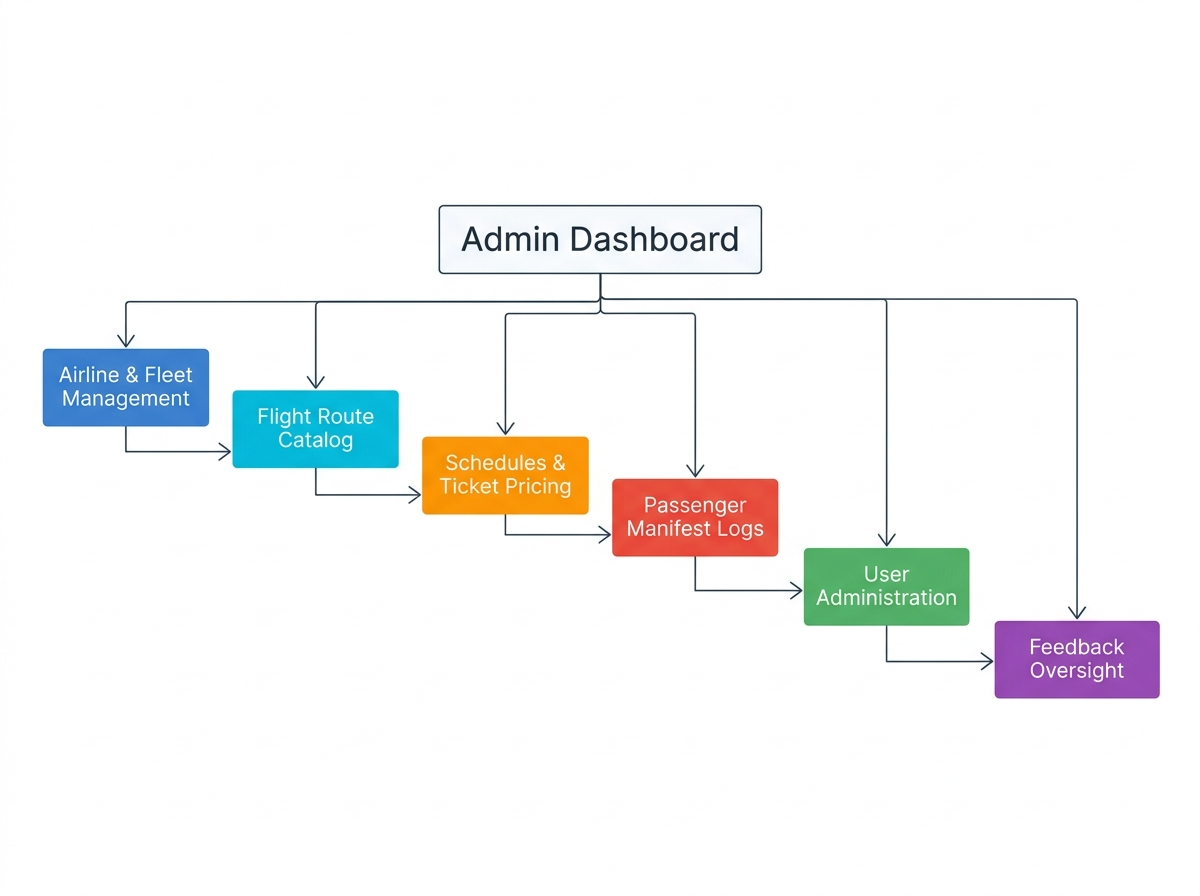
\includegraphics[width=0.9\textwidth]{images/admin_flow_chart.jpg}
\caption{Administrative Portal Operations & Module Routing Layout}
\label{fig:admin_modules}
\end{figure}

The primary administrative screens and modules are structured as follows:
\begin{enumerate}
    \item \textbf{Airlines \& Fleet Manager} (\texttt{AirlineManagement.jsx}, \texttt{AddAirline.jsx}): Admin users can register carriers, specify flight prefix codes (e.g., SG, AI), and track fleet sizes.
    \item \textbf{Flight Catalog Manager} (\texttt{FlightsManagement.jsx}, \texttt{AddFlight.jsx}): Defines core flight routes, selecting origin and destination terminals, and binding them to flight numbers.
    \item \textbf{Schedule \& Pricing Planner} (\texttt{Schedule.jsx}, \texttt{Update.jsx}): Allocates scheduled flights on specific dates. Admins can update ticket pricing grids and cabin seat configurations.
    \item \textbf{Passenger Manifest Tracking} (\texttt{Bookings.jsx}, \texttt{PassList.jsx}, \texttt{PassInfo.jsx}): Accesses real-time lists of flyers booked on specific flight numbers, sorted by date.
    \item \textbf{User Administration} (\texttt{UserInfo.jsx}): Lists user accounts and active profiles. Includes account status toggles to enable or disable profiles.
    \item \textbf{Feedback Oversight} (\texttt{Feedbacks.jsx}): Reviews ratings and comments submitted by travelers.
\end{enumerate}

\newpage
\section{Security, Safety, \& Crash Protections}
To achieve commercial viability, the application implements safety configurations across both frontend and backend layers:

\subsection{Backend Crash Prevention Systems}
To prevent server crashes, global process listeners are initialized at boot inside \texttt{server.js} to handle unhandled errors:
\begin{lstlisting}[language=javascript]
process.on("uncaughtException", (err) => {
  console.error("Uncaught Exception caught:", err.message);
});

process.on("unhandledRejection", (reason) => {
  console.error("Unhandled Rejection caught:", reason?.message || reason);
});
\end{lstlisting}
This prevents unexpected server crashes in the event of database timeouts or socket drops.

\subsection{Robust Stripe Fallback Integration}
To ensure the application remains operational during testing or offline runs without a valid Stripe secret key, the server catches payment initiation exceptions and provides a fallback structure:
\begin{lstlisting}[language=javascript]
app.post("/api/payments", async (req, res) => {
  try {
    // Attempt Stripe Checkout creation...
  } catch (error) {
    console.error("Payment error:", error.message);
    res.status(500).json({ error: error.message });
  }
});
\end{lstlisting}
If the API returns a status 500 or error code, the frontend client intercepts the response, alerts the user that it is running in sandbox test mode, and redirects them to the boarding pass output screen.

\subsection{Form Field Style Safeguards}
All input forms are styled with text contrast overrides (\texttt{text-slate-900}) to ensure text remains clearly visible when filling forms on bright screens.

\subsection{Routing Constraint Filters}
The search widget utilizes validation filters preventing matching origin and destination parameters (e.g. searching DEL to DEL is blocked).

\section{Web Application Interface \& Screenshots}
This section outlines the visual interfaces developed for the Flyhigh platform. Users can integrate actual system screenshots by saving images (e.g., \texttt{home\_page.png}, \texttt{boarding\_pass.png}, \texttt{admin\_dashboard.png}) in their local working directory and uncommenting the associated \texttt{\textbackslash includegraphics} commands:

\begin{figure}[htbp]
\centering
% 
\includegraphics[width=0.9\textwidth]{home_page.png}
\begin{center}
\framebox(360,180){Placeholder: Home Page Flight Search Widget (\texttt{home\_page.png})}
\end{center}
\caption{Flyhigh Landing Page \& Glassmorphic Flight Search Panel}
\label{fig:ss_home}
\end{figure}

\begin{figure}[htbp]
\centering
% \includegraphics[width=0.9\textwidth]{boarding_pass.png}
\begin{center}
\framebox(360,180){Placeholder: Print-Ready Boarding Pass (\texttt{boarding\_pass.png})}
\end{center}
\caption{Dynamic Boarding Pass Stub with Barcode Elements}
\label{fig:ss_pass}
\end{figure}

\begin{figure}[htbp]
\centering
% \includegraphics[width=0.9\textwidth]{admin_dashboard.png}
\begin{center}
\framebox(360,180){Placeholder: Admin Dashboard (\texttt{admin\_dashboard.png})}
\end{center}
\caption{SSO Administrative Interface \& Metrics Control Panel}
\label{fig:ss_admin}
\end{figure}

\section{Conclusion \& Future Roadmap}
The developed \textbf{Flyhigh} platform successfully integrates client-facing booking components with administrative controls. Future roadmap enhancements include:
\begin{itemize}
    \item \textbf{JWT Authentication Integration}: Replacing basic session checks with secure JSON Web Token authorization headers.
    \item \textbf{Interactive Seating Charts}: Implementing an SVG seat-mapping interface to let users select specific seats.
    \item \textbf{SMTP Mail Notifications}: Utilizing Nodemailer to dispatch confirmation e-tickets automatically on checkout.
\end{itemize}

\end{document}
